\documentclass{article}
\usepackage[utf8]{inputenc}
\usepackage[T1]{fontenc}
\usepackage[francais]{babel}
\usepackage{textcomp}
\usepackage{amsmath,amssymb,amsthm}
\usepackage{lmodern}
\usepackage[a4paper]{geometry}
\usepackage{graphicx}
\usepackage{xcolor}
\usepackage{multicol}
\usepackage{microtype}
\usepackage{pdfpages}
\usepackage{listings}
\usepackage{color}
\usepackage{appendix}


\usepackage{hyperref}
\hypersetup{pdfstartview=XYZ}
 

\usepackage{fancyhdr}
\pagestyle{fancy}
\renewcommand\headrulewidth{0.4pt}
\fancyhead[L]{Le Cesne Benjamin - Tardy Luca}
\fancyhead[R]{Prep'ISIMA / L2 INFO}
\renewcommand\footrulewidth{0.4pt}
\fancyfoot[C]{
\textbf{Page \thepage/5}}
\fancyfoot[L]{\textit{Projet - Prep'ISIMA}}
\fancyfoot[R]{\today}
\newcommand{\variable}[1]{\texttt{#1}}

\definecolor{darkWhite}{rgb}{0.92,0.92,0.92}

\lstset{frame=single,
  language=C,
  showstringspaces=false,
  columns=flexible,
  backgroundcolor=\color{darkWhite},
  basicstyle={\small\ttfamily},
  numbers=left,
  numberstyle=\tiny\color{black},
  framexleftmargin=20pt,
  framexrightmargin=20pt,
  keywordstyle=\color{blue},
  commentstyle=\color{red},
  stringstyle=\color{violet},
  breaklines=true,
  breakatwhitespace=true,
  tabsize=2,
}


\begin {document}
\hfill
\hfill
\hfill
\begin{center}
  \large{PROJET EULER}

  Problème 119
\end{center}
\tableofcontents
\section {Résolution du problème}
\subsection {Présentation du problème}

Le problème 119 du Projet Euler consiste à trouver le 30ème nombre tel que la somme de ses chiffres élevé à une certaine puissance soit égale à lui-même. Par exemple, le 1er nombre respectant ces règles est 81 car la somme des chiffres de 81 est : $ 8 + 1 = 9 $ et $ 9^{2} = 81 $. De même, le deuxième est 521 : $ 5 + 2 + 1 = 8 $ et $ 8^{3} = 521 $	. Dans l'énoncé du problème, on nous dit que le dixième est 614 656. On rappelle qu'un nombre doit contenir au moins deux chiffres pour avoir une somme.

\subsection{Méthodes de réflexion}

\subsubsection{Méthode itérative}

Une première méthode pour calculer la somme des chiffres d'un nombre consiste à récupérer le reste de la division du nombre par 10, de l'ajouter à la somme puis faire la division entière de notre nombre par 10 et répéter ceci jusqu'à ce qu'il soit égal à 0. Par exemple, pour 614 656, le reste de $614656/10$ est 6 et la division entière de 614 656 par 10 donne 61 465. Ensuite le reste de $61465/10$ est 5. Ainsi de suite, on obtient $6 + 5 + 6 + 4 + 1 + 6$. Ici, on divise 6 par 10, ce qui donne 0 et qui cause la sortie de la boucle. On a donc bien obtenu la somme des chiffres de 614 656.
\newline

Pour trouver le 30ème nombre respectant les règles citées précédemment, il existe une méthode itérative, vérifiant pour chaque nombre, en partant de 10, s'il fait partie des nombres que l'on recherche. Ainsi, pour chaque nombre, on calcule la somme de ses chiffres, on l'élève au carré (on appelera ce nombre $n$), on vérifie si le résultat est égal au nombre de départ, auquel cas on ajoute 1 à un compteur qui doit atteindre 30. Si $n$ est inférieur au nombre de départ, on augmente la puissance et on recommence, s'il est supérieur on s'arrête car il ne pourra plus jamais être égal au nombre de départ, et on passe au nombre suivant. Lorsque le compteur atteint 30 c'est qu'on a trouvé le nombre que l'on cherche. Or, cette méthode est beaucoup trop longue car l'ordre de grandeur du 30ème est de $10^{15}$, sachant que l'on calcule la somme des chiffres de tous les nombres précédent. D'après nos calculs, la complexité en temps de cette méthode est en $O(e^{n})$  où $n$ est le nombre de chiffres du nombre que l'on recherche.


\subsubsection{Seconde méthode}

Cette seconde méthode ne consiste pas à réduire la complexité de notre fonction qui calcule la somme des chiffres d'un nombre mais plutot d'atteindre plus rapidement le 30ème sans avoir à calculer la somme des chiffres de tous les nombres. Pour cela, nous pouvons prendre des petits nombres $a$ (par exemple jusqu'à 400 pour commencer) que l'on éléve à des petites puissances $b$ (par exemple jusqu'à 50 pour l'instant) et calculer la somme des chiffres de chacun de ces nombres $a^{b}$. Lorsque $a^{b} = a$, on ajoute ce dernier à une liste. Après avoir testé tous les nombres, on trie la liste pour en récupérer le 30ème. De cette façon, on calcule la somme des chiffres de beaucoup moins de nombre puisqu'il y en a une multitude qui ne sont pas une puissance d'un autre. Par exemple, aucun nombre élévé à une certaine puissance est égal à 26 donc on ne calcule jamais la somme des chiffres de 26. Ceci réduit clairement le temps d'éxécution de notre programme et nous avons réussi à trouver le nombre recherché qui est 248 155 780 267 521.

\subsection{Le problème du "J'ai de la chance"}
Malheureusement, cette méthode a posé un autre problème. Si l'on veut développer un programme générique qui pourrait retourner un nombre quelconque de la liste de ceux qui respectent les règles, il faut compter sur la chance. En effet, dans notre cas, nous avons décider d'aller jusqu'a $400^{50}$ et heureusement nous avons trouvé le bon résultat. Mais rien ne nous disait auparavant que le nombre que l'on cherchait n'était pas égal à $500^{10}$ ou $5^{75}$ (sachant que ces deux nombres sont plus petits que $400^{50}$ mais que nous ne les testons pas). Si c'était le cas, notre programme n'aurait pas renvoyé le bon résultat puisqu'il ne l'aurait même pas étudié donc pas ajouter à la liste. C'est ainsi qu'on s'est demandé s'il n'y avait pas un moyen de connaître à l'avance le $a$ et le $b$ maximum pour lesquels le programme donne le bon résultat.

\section {Optimisation}
\subsection {Rappels de nos objectifs}
Suite à notre dernier entretien, nos objectifs sont les suivants :

- Etudier la piste du logarithme afin de déterminer à l'avance nos bornes de recherche

- Déterminer les limites de notre fontion qui calcule la somme des chiffres d'un nombre

- Essayer de supprimer ce phénomène de chance dans notre programme

\subsection{Comment trouver les bornes de recherche ?}

Ici, notre objectif est de borner $a$ et $b$ de manière à ce que $a^{b}$ soit inférieur à un certain nombre défini à l'avance. Ainsi, on considère que lorsque l'on cherche le n-ième terme de notre liste de nombres, on connait approximativement son ordre de grandeur et il existe une valeur connue, supérieure à cette dernière. Si on appelle $vMax$ cette valeur maximum, le but est donc de trouver pour quelles valeurs de $a$ et de $b$, $a^{b}  < vMax$.

\subsubsection{Comment borner a ?}

	Nous devons trouver la valeur maximum de $a$ telle que $a^{b} < vMax$. Pour cela, il faut prendre la valeur minimum de $b$, car $\forall a1, a2, vMax, b1, b2 \in \mathbb{R}, b1 > b2 \Rightarrow \exists a1 > a2, a2^{b1} > a1^{b2}$.

Ainsi, on obtient l'inéquation suivante : \[ a^{2} < vMax \]
 \[ \Leftrightarrow \ln{a^{2}} < \ln{vMax} \]
\[ \Leftrightarrow 2*\ln(a) < \ln(vMax)  \]
\[ \Leftrightarrow \ln(a) < \frac{\ln(vMax)}{2}  \]
\[  \Leftrightarrow a < e^{\frac{\ln(vMax)}{2}} \]

Ainsi, si l'on connaît $vMax$, on sait à l'avance que $a$ ne devra pas dépasser $e^{\frac{\ln(vMax)}{2}}$


\subsubsection{Comment borner b ?}

Une fois que l'on connaît la valeur maximum de $a$, on peut exprimer la valeur limite de $b$ en fonction de $a$ et de $vMax$. On a donc l'inéquation suivante :  \[ a^{b} < vMax \]
 \[ \Leftrightarrow \ln{a^{b}} < \ln{vMax} \]
\[ \Leftrightarrow b*\ln(a) < \ln(vMax)  \]
\[ \Leftrightarrow b < \frac{\ln(vMax)}{\ln{a}}  \]

Ainsi, si l'on connaît $vMax$ et $a$ , on sait à l'avance que $b$ ne devra pas dépasser $\frac{\ln(vMax)}{\ln{a}}$

\subsection{Optimisation de la fonction qui calcule la somme des chiffres d'un nombre ?}

Lorsque l'on borne $a$ et $b$, le temps de calcul augmente largement car en supprimant la chance de notre programme on augmente largement le nombre d'appels à la fonction sommeChiffresNombre afin d'être sûr de trouver le bon résultat. Nous avons donc essayé de réduire le temps de calcul de cette fonction, d'autant plus que celle-ci ne fonctionne plus à partir d'une certaine valeur. En effet, nous n'avons pas réussi à en connaître la raison mais à partir de $10^{17}$ notre fonction ne retourne pas le bon résultat. Nous avons donc essayé une différente méthode pour calculer la somme des chiffres d'un nombre et cette dernière s'est retrouvé beaucoup plus efficace, pas tellement au niveau du temps de calcul mais plus au niveau de la complexité et du fait qu'elle fonctionne pour toutes les valeurs. Elle consiste à transformer le nombre en chaîne de caractères et calculer la somme des caractères de la chaîne obtenue. En python, la fonction correspond donc à :
\begin{lstlisting}
def sommeChiffreNombre(nombre):
    return sum([ int(c) for c in str(nombre) ])
\end{lstlisting}

\subsection{Comment déterminer vMax ?}

Pour pouvoir borner $a$ et $b$, il faut d'abord déterminer $vMax$. Le temps d'exécution dépendra de $vMax$ car si il est trop éloigné de la valeur recherchée, le temps d'exécution du programme sera trop élevé. Cependant, on ne peut connaître à l'avance la valeur recherchée. C'est pourquoi nous avons fait en sorte d'augmenter progressivement $vMax$ : si $vMax$ est atteint sans que l'on ait trouvé le $n^{eme}$ terme (où le $n^{eme}$ terme est celui que l'on recherche), on augmente $vMax$. La formule que nous avons choisit pour augmenter $vMax$ est : \[vMax = vMax * 5^{(n^{ème} terme - \text{la quantité déjà trouvé})/2}\] Cette formule n'est pas admise mais résulte de nos expériences. Par exemple : on cherche le 20ème terme, et on en a déja trouvé 10 avec le $vMax$ actuel. Ici, $n^{eme} terme - \text{la quantité déjà trouvé} = 10$. On multiplie donc $vMax$ par$5^{5}$ ($5^{10/2}$). Ainsi, peu importe le $vMax$ d'origine, le programme finira toujours pas trouvé la solution. Néanmoins il existe des $vMax$ plus efficaces pour certaines valeurs. Par exemple : la valeur recherchée est $1 000 000$ et le $vMax$ d'origine est $2$. Admettons que $vMax$ atteigne $999 999$, le programme n'aura pas trouvé la bonne valeur mais $vMax$ augmentera de beaucoup trop pour rien. Alors que si le $vMax$ d'origine avait été égal à $3$, on aurait atteint plus rapidement et simplement $1 000 000$. On remarque donc que le programme est plus rapide pour $vMax = 2$ que pour $vMax = 3$, même s'il fonctionne dans les deux cas. Ce n'est ici qu'un exemple, et en suivant les contraintes de ce problème, on peut déterminer un palier : si $n < 10$, il faut choisir $vmax = 10$, sinon il faut commencer avec $vMax = 700 000$.

\section{Comparaison des deux méthodes}
Afin de comparer l'efficacité de nos deux méthodes nous avons réaliser un tableau représentant le temps d'exécution de nos deux programmes en fonction de la valeur recherchée avec le même $vMax$ à chaque fois :

\bigbreak
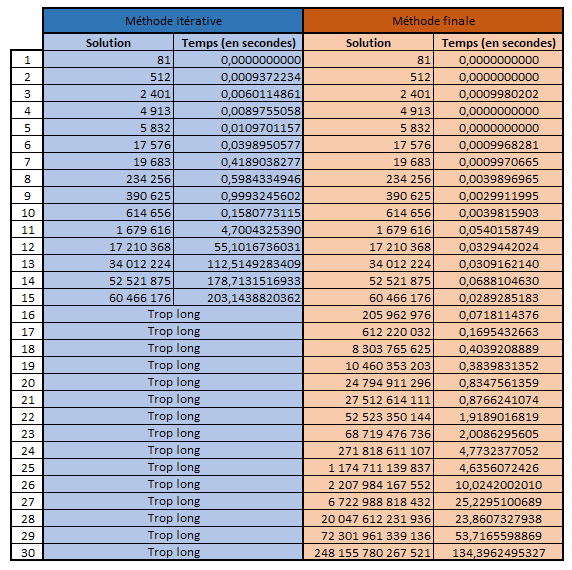
\includegraphics[width = 8cm]{Tableau.png}
\bigbreak

Ainsi, grâce à ce tableau, nous remarquons qu'à partir du 12ème terme, le temps d'exécution de la première méthode devient plus de 1000 fois supérieur à celui de la seconde. De plus, à partir du 16ème terme, la première méthode devient beaucoup trop long pour être mesuré. L'efficacité de la seconde méthode par rapport à la première est donc avéré puisqu'elle met autant de temps à trouver le 30ème terme que la première pour trouver le 13ème.

Nous avons aussi réaliser un graphique représentant l'évolution de ces temps d'exécution en fonction du terme recherché :

\bigbreak
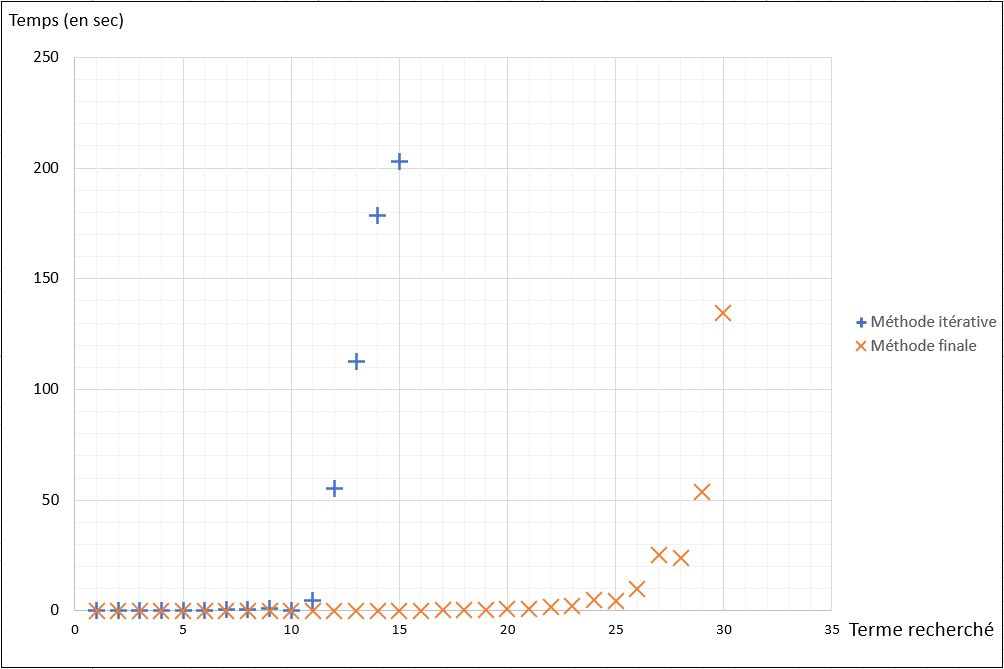
\includegraphics[scale = 0.5]{Graphe.png}
\bigbreak

Ici, nous voyons bien que pour les deux méthodes, le temps d'exécution devient exponentiel à partir d'un certain point. Ce dernier est beaucoup plus grand pour la seconde méthode ce qui explique sa meilleure efficacité.

\begin{appendix}

\end{appendix}


\end{document}
